\documentclass[9pt,twocolumn,twoside]{../../styles/osajnl}
\usepackage{fancyvrb}
\journal{i524} 

\title{Hadoop YARN}

\author[1,2]{Milind Suryawanshi}
\author[1,*]{Gregor von Laszewski}

\affil[1]{School of Informatics and Computing, Bloomington, IN 47408, U.S.A.}
\affil[2]{Savitribai Phule Pune University 2010, Pune, Maharashtra 411007 India }

\affil[*]{Corresponding authors: laszewski@gmail.com}

\dates{project-paper2, \today}

\ociscodes{Hadoop, Yarn, MapReduce, Cluster}

% replace this with your url in github/gitlab
\doi{\url{https://github.com/MilindSuryawanshi/sp17-i524/tree/master/paper2/S17-IO-3020/report.pdf}}


\begin{abstract}
Apache Hadoop 2.0 came up with Yarn architecture which is capable of managing resources and processing of tasks separately. This is the most important implementation over MapReduce which increased the scalability of Hadoop 1.0. YARN is the next generation of Hadoop's compute platform.

\end{abstract}

\setboolean{displaycopyright}{true}

\begin{document}

\maketitle

\section{Introduction}

Apache Hadoop \cite{www-7} is open source software framework, can be installed on a cluster of computers, which can communicate together for large amount of data storage and processing it, in highly distributed manner. Hadoop 2.0 project was developed to resolve the limitations of MapReduce (we will see the limitation as we move ahead). YARN (Yet Another Resource Negotiator) is Apache Hadoop’s cluster resource management system \cite{www-1}. It’s a resource management technology which makes pace between, the way applications use Hadoop system resources and node manager agents. To understand Yarn, it is important to know the limitation of Hadoop1.0 MapReduce, which enforced the creation of Hadoop 2.0. Hadoop 2.0 alpha version introduced in August 2013 \cite{www-8}.


\section{Limitation of MapReduce}

Hadoop 1.0 was designed for big data processing and MapReduce was the only option supported.MapReduce is the Hadoops framework, which Maps the multi terabyte data sets into chunks which will getting executed in parallel manner. The sorted output of the Map then given to Reduce tasks \cite{www-6}. In MapReduce framework Node holds the meta data information and the daemon Job Tracker will be ensuring that the Task Tracker are processing the data. Task Tracker runs the Map and reduces the tasks and reports the status to Job Tracker. Job Tracker tracks the tasks, schedules the jobs and monitors the Tasks Tracker. As shown in figure 1, Job Tracker performs multiple operations which is bottleneck as we keep increasing the number of Task Trackers. Maximum 4000 Task Tracker and 40,000 concurrent tasks, can be handled by single Job Tracker. This was causing the limitation on use of number of Tasks Trackers. In MapReduce, there was a hard partition on resource utilization, which was causing inefficient use of resources \cite{www-3}.

\begin{figure}[htbp]
	\centering
	\fbox{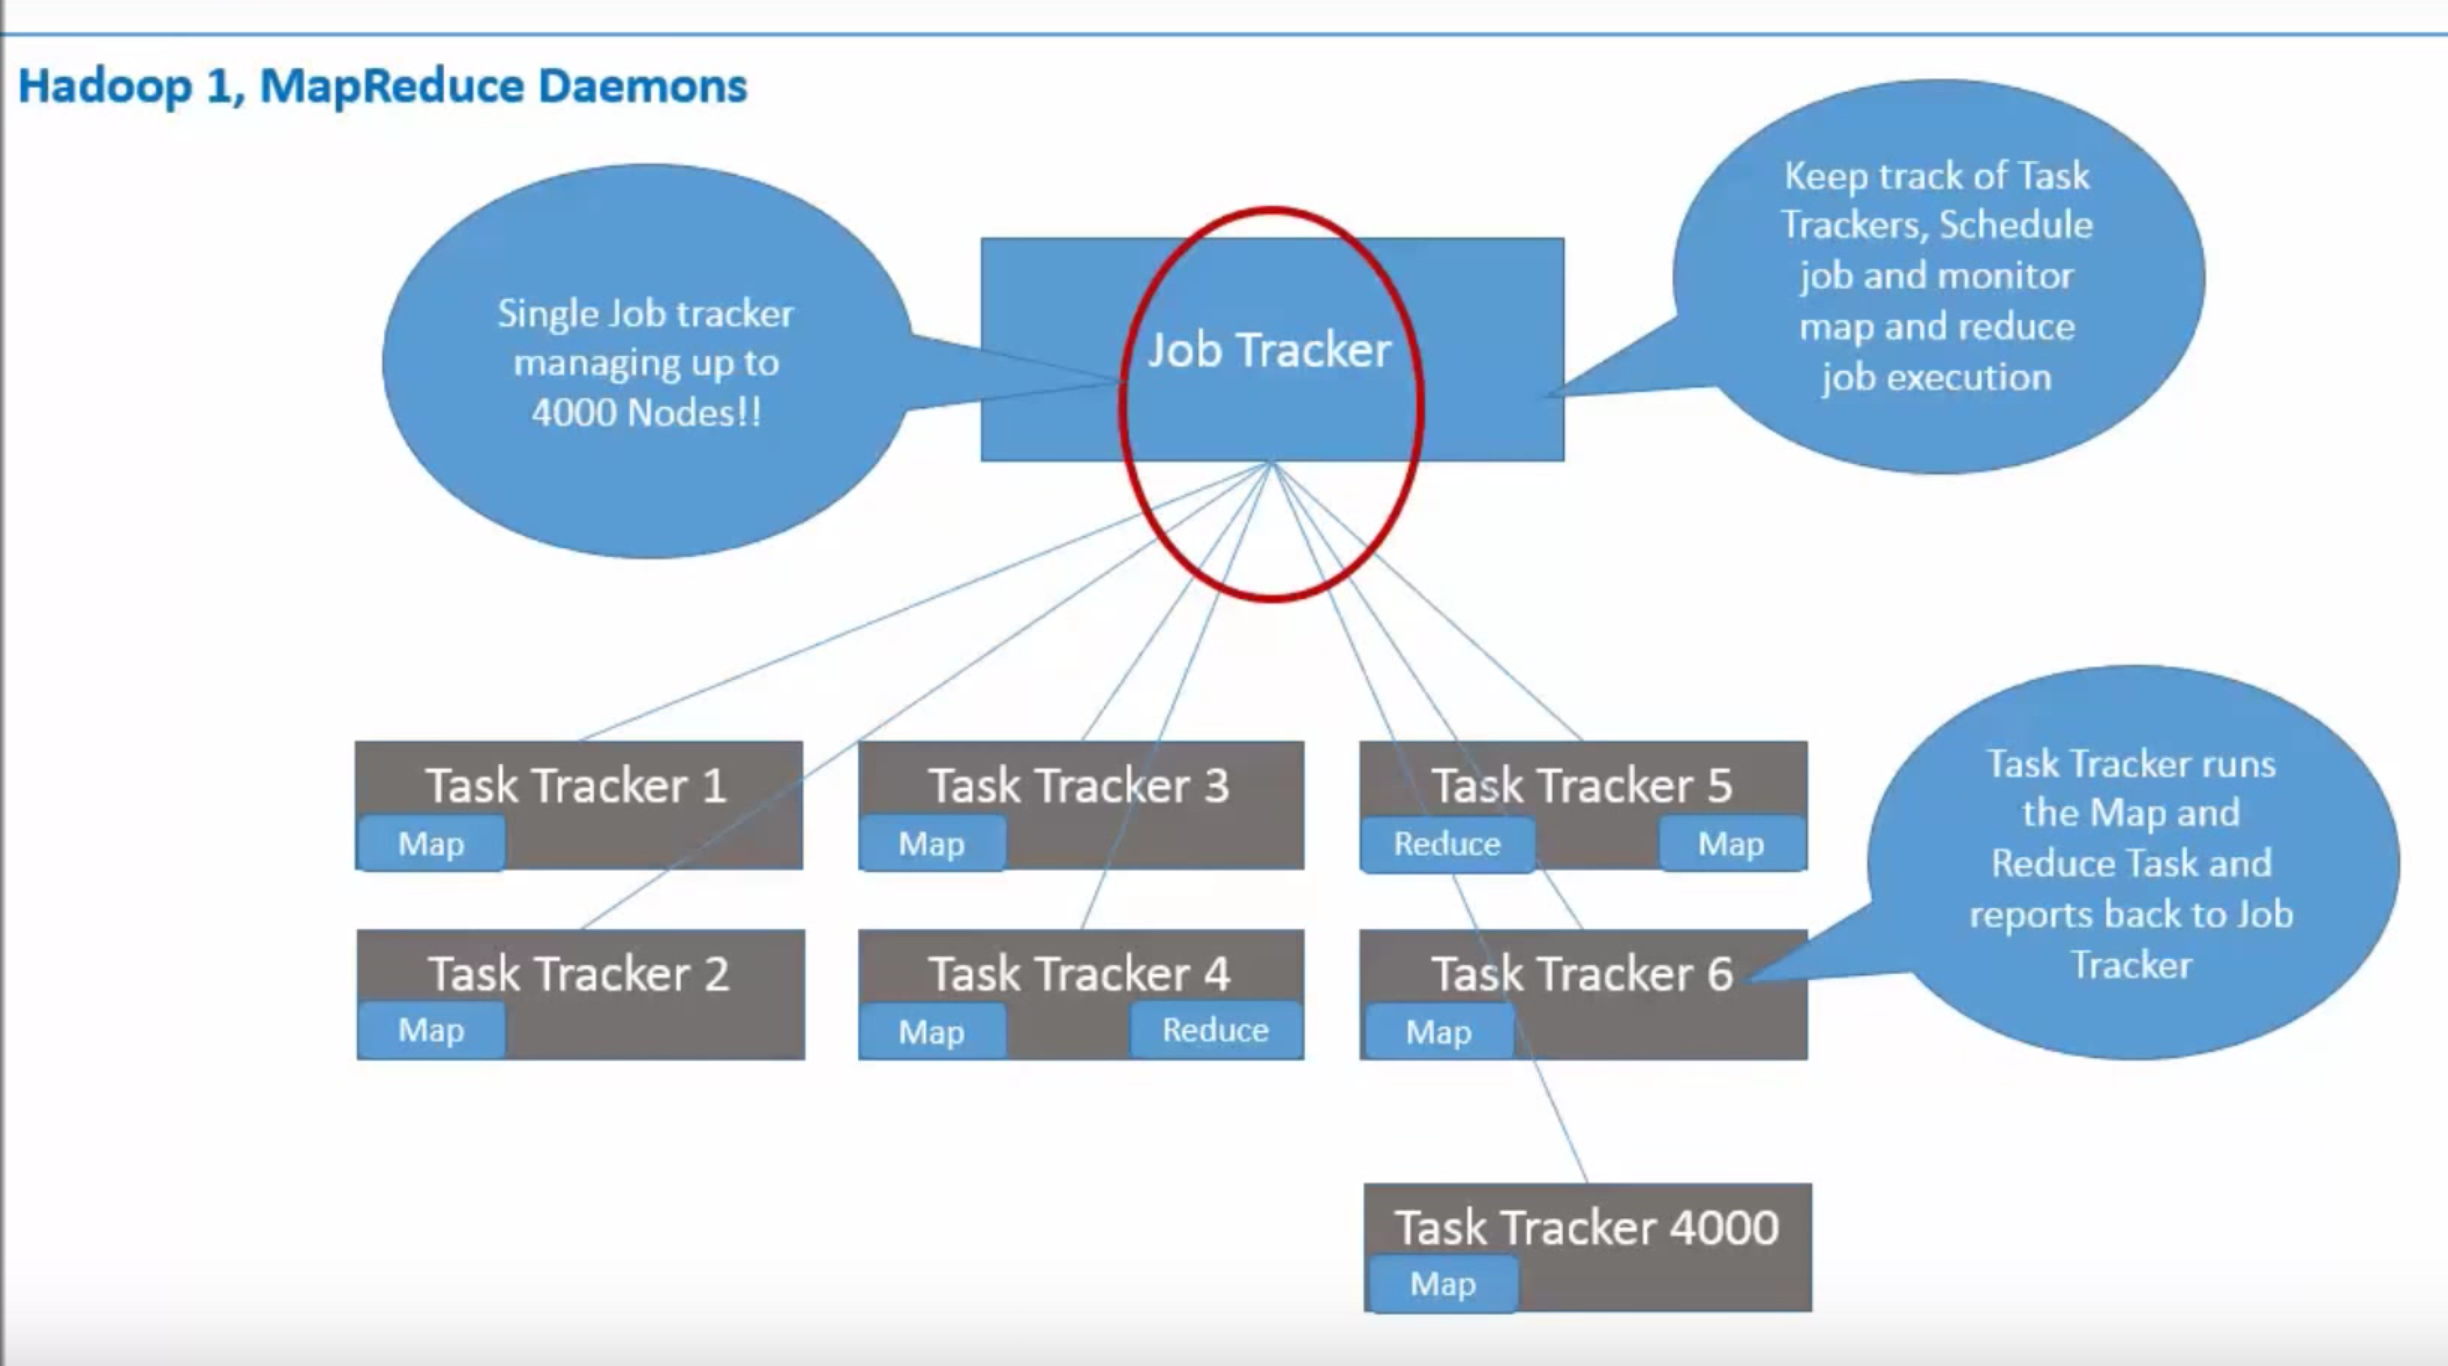
\includegraphics[width=\linewidth]{images/Hadoop1_0}}
	\caption{Hadoop 1, MapReduce deamon diagram \cite{www-3}. }
	\label{fig:false-color}
\end{figure}


\section{Design}
To overcome the limitation of MapReduce, Hadoop 2.0 was introduced with Yarn. Yarn is an architectural center of Hadoop 2.0 design \cite{www-4}. It allows multiple data processing engines like Batch Streaming \cite{www-3}, Interactive SQL \cite{www-3}, Data science and Real time streaming to store and retrieve data in Hadoop Distributed File System (HDFS). Figure 2 showing the Hadoop 2.0 architectural design. Yarn is pre-requisite to Enterprise Hadoop. It acts as middle layer in Hadoop cluster which extends the Hadoop capability which provides resource management, delivers consistent operation, security and data governance tools across Hadoop cluster. It provides ISV engines with a consistent framework which allows developer to write data access applications that run in Hadoop. ISV’s (in a context of Hadoop Yarn) create the software product to support and run on the Hadoop Yarn architecture.  

\begin{figure}[htbp]
	\centering
	\fbox{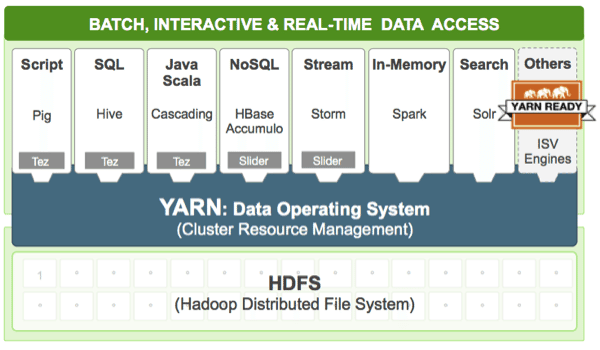
\includegraphics[width=\linewidth]{images/YARN_design}}
	\caption{Architecture diagram for Hadoop 2.0 Yarn\cite{www-4}. }
	\label{fig:false-color}
\end{figure}

\section{Architecture}
Apache Hadoop YARN architecture has ResourceManager, ApplicationManager, NodeManager and distributed application as its important parts. Figure 3 shows the architectural work flow of Yarn. YARN’s global ResourceManager runs in a master daemon. Usually ResourceManager is placed in dedicated machine, it allocates the requested resource based on available cluster resources. It keeps track of how many live nodes and resources are available on cluster for allocation. It coordinates with the NodeManager for resource allocation and release functionality. ResourceManager consists of two major components Scheduler and ApplicationManager \cite{www-2}. 
Scheduler is pure scheduler which only allocates the resource, it will not perform any monitoring or tracking of status. Scheduler schedules the resource (like cpu, disk, network etc.) based on applications requirement. Scheduler can divide the cluster resource among the application tasks, queues it is called as pluggable policy \cite{www-2}. Once user submits the application to the ResourceManager, the ResourceManager’s scheduler will allocate the resource to it. Once resource get allocated ApplicationManger comes into picture and perform the coordination all the tasks running for that application like: monitoring of tasks, restarting failed tasks, speculatively running slow tasks and total values of application counter. It also asks for appropriate resources to run tasks \cite{www-4}. This work flow is shown in figure 3.

\begin{figure}[htbp]
	\centering
	\fbox{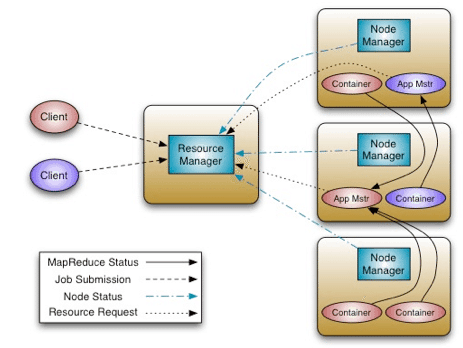
\includegraphics[width=\linewidth]{images/YARNArch}}
	\caption{Hadoop 2.0 Yarn architectural workflow diagram \cite{www-1}. }
	\label{fig:false-color}
\end{figure}

NodeManager will create the container to perform the given tasks. Container size depends on the tasks he needs to perform. Container can be any resource type like CPU, disk, network, and storage. NodeManger can have number of containers depending on the configuration parameter and node resource capacity. 
Each application has its ApplicationManager. It performs required tasks inside a container. E.g. the MapReduce. ApplicationMaster performs the map and reduce tasks. On similar line Giraph’s ApplicationMaster perform Giraph specific tasks in a container. The ResourceManger, the NodeManager and a container work regardless of the type of application. This Yarn feature, makes it more popular, as this allows to run different types of application in a single cluster. This generic approach allows Hadoop Yarn cluster to run various application like MapReduce, Giraph, Storm, Spark, Tez/Impala, MPI etc. To understand the popularity of the Hadoop Yarn, we need to know its advantages.

\subsection{Advantages} 
\begin{itemize}
	\item Resources can be shared among different clusters, which maximizes the efficiency of resource utilization.
	\item All in one cluster will help to run maximum application, will reduce the operation cost.
	\item Reduce the data transfer operation, as there is no need to transfer the data between Hadoop Yarn and system running on different clusters of machine \cite{www-4}.
\end{itemize}
	
\section{Feature}

Yarn came with lots of features; we are not covering each of the features here. However, this article will be covering the most important feature, compared to MapReduce, which makes Yarn popular \cite{www-4}.

\begin{itemize}
	
	\item \textbf{Uberization:}  To reduce the overhead on ResourceManager, a small tasks container can ask NodeManager to start their tasks. So all the small tasks of MapReduce are run by ApplicationMaster’s JVM. This improves the performance.

	\item \textbf{Multi-tenancy:}  Yarn allows multiple engines to access the Hadoop as a common platform for batch processing, interactive and real time data access. This feature returns the most enterprise investment for business.
		
	\item \textbf{Cluster Utilization:}  This feature overcomes the limitation of not using hardware resource efficiently for jobs in MapReduce. Yarn dynamically allocates the resource which improves the resource utilization. 

	\item \textbf{Scalability:}  Introduces cluster manager so ResourceManager can solely focus on scheduling and let cluster to track the live nodes and available resources in the cluster and assign the tasks to them. 
	
	\item \textbf{Computability:} Existing MapReduce application can run on the latest Hadoop2 Yarn, without failing. 

\end{itemize}	
	
\section{Limitation}

	Any new offering takes time to mature and align with market expectation. There are following limitations of Yarn. As the product is growing it is coming with better ecosystem to overcome its limitation \cite{www-5}: 
\begin{itemize}	
	
	\item Complexity  
		\begin{itemize}	
			\item Yarn is complex and level of abstraction is low, from the perspective of developers. 
			\item Developers need to do very low level tasks, for example:  a Hello World program is of 1500 lines code.
			\item Clients need to be prepared with all the dependencies (it is mostly library files which help the current program to run with additional functionality).
			\item To up and run the app, client requires to setup the environment, like class path. 
			\item To see the log, developer needs to wait till completion of the job, currently there is no mechanism to show the console log while the job is running.	
		\end{itemize}		
		

	\item Application cannot handle the master crash, which causes the single point failure of the app
	\item There is no \textit{built in} communication layer available between master and container.
	\item Not helpful in long running Jobs
	\item Hard to debug
	
\end{itemize}
	
\section{Conclusion}

Apache Hadoop Yarn is important part of Hadoop 2.0 architecture, which separates the resource management and processing components. With this functionality it achieves scalability, efficiency and flexibility compared to MapReduce engine (from first version of Hadoop). Adding to this Yarn based architecture will not limit the existing MapReduce applications. It supports such existing application to run in Hadoop 2.0, without failure. Most of the Hadoop 1.0 users are migrating to Hadoop 2.0. Yarn runs the large scale data, Yahoo deployed 35,000 nodes for 6 months without failure. Yarn allows multiple access engines like Pig, Hive, JavaScala, NoSQL, Spark and also engines from independent vendor to use the HDFS using Hadoop Yarn. This increased the Hadoop Yarn compatibility to larger extend. YAHOO!, eBay, Spotify, Xing, Allegro and more are already using the Hadoop Yarn.


\section*{Acknowledgements}

Special thanks to Professor Gregor Von Laszewski for giving me an opportunity to write this paper and the most valuable suggestions. Also the entire class and TA’s for their suggestion and support.

% Bibliography

\bibliography{references}
 
\end{document}
